\chapter{Evaluation of the First Two Implementations}

\begin{quote}
``Inspiration may be a form of super-consciousness, or perhaps of sub consciousness, I wouldn't know. But I am sure it is the antithesis of self-consciousness.'' �- Aaron Copland
\end{quote}

\noindent In this chapter, we will evaluate the Mapping and L-System implementation with a carefully considered strategy. This strategy will place special emphasis on the main problem posed by this project; that \textbf{music is subjective}.

\section{How Can an Objective Evaluation be made of a Subjective Concept?}

Recall that we looked briefly at the concepts of \textbf{music cognition}. From these concepts, we understood that sound is ``processed'' into music by a human based on their personal experience. In other words; music is subjective.

How can we describe aspects of an account that will present themselves through the generated music? How can we ensure that these aspects are described in a way that \textit{both} represent the aspects of the account \textit{and} corresponding aspects of the music that relate to the account?

To help answer this, a simple analysis of publications such as \textit{The Financial Times} is called for. A browse through will reveal a surplus of buzz-words which can be used to describe aspects of an account (figure: \ref{fig:wordcloud}). An accountant who is looking at an accountant will develop an overall impression of an account. They can then describe it to a novice using a selection of these words. A novice, with little understanding of accountancy, can then understand the overall state of the account. These buzz-words are both accessible to an expert accountant, and a novice.

\begin{figure}[ht]
\centering
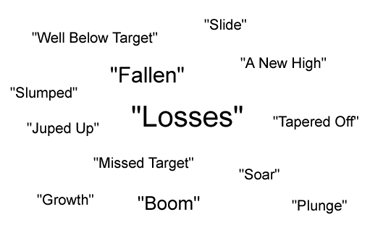
\includegraphics[scale=0.75]{word_cloud}
\caption{This word cloud shows how frequently some buzzwords occur in financial articles. The larger the font size, the greater the word's frequency.}
\label{fig:wordcloud}
\end{figure}

As an example, consider a company with vastly increasing debts and vastly decreasing profit. We give this company's balance sheet to an expert to analyse. Their experience allows them to perceive the dire state of this company, and choose the word ``plunge'' to describe the company's state.

Now consider that we generate music from this account using one of the strategies developed in previous chapters. This music is played to someone who has not seen the balance sheet. What they might hear is a lot of descending scales in a minor key quickly moving downwards. They may well also choose to describe this as a ``plunge''. It is this \textbf{synchronisation} of descriptions that we are looking for when we evaluate the approaches.

Therefore it is these buzz-words that will be the key to bridging the descriptive gap between the accounts and the generated music.

\section{Human Factors}

In the previous chapter, we briefly mentioned the issue of \textbf{listening fatigue}. If the tester's concentration lapses during the testing, they will have the opportunity to play a sequence again. They will also have the opportunity to take breaks during the testing process. Additionally, sequence length are limited to a maximum of 20 seconds, and the whole testing process is intended to take no longer than 20 minutes.

\section{Preparation of Test Data}

Fifteen accounts were sent to the expert to be evaluated. From these, \textbf{six were chosen}. Of these, \textbf{Three} were selected which displayed mostly \textbf{desirable aspects} (good investment proposition), and \textbf{Three} were selected which displayed mostly \textbf{undesirable aspects} (bad investment proposition).

From the approaches, \textbf{four methods} of generating music were chosen. From the \textbf{Signal Mapping} approach, music was generated both in \textbf{sequence} and in \textbf{parallel}. And, from the \textbf{L-System} approach, music was generated firstly with \textbf{strings and piano} and then with \textbf{piano only in staccato}.

This results in a total of 24 generated musical sequences which were prepared for evaluation. These musical sequences were then \textbf{shuffled randomly}.

\section{Designing an Evaluation Strategy}

With most testing strategies, a baseline is needed which can be used as a fixed point for comparing data. For this, an accountant was asked to analyse 16 accounts (A sample of the questionnaire that the accountant received can be seen in \textit{figures \ref{fig:qa1}, \ref{fig:qa2} and \ref{fig:qa3}} of the appendix).

The accountant was asked to choose a selection of terms to describe the \textit{account}, and were also asked to state whether they would invest in the company based on what they'd seen (they could select `yes', `no' or `unsure').

\begin{figure}[ht]
\centering
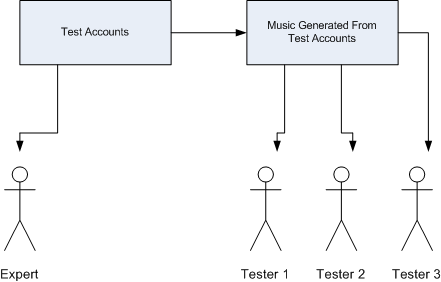
\includegraphics[scale=0.7]{testing.png}
\caption{A diagram showing how the evaluation process is organised.}
\label{fig:testing.png}
\end{figure}

For the testers who would be listening to the music, they will have to choose a selection of terms to describe the \textit{music}, and also make an assessment as to whether they'd invest in the company or not (A sample of the questionnaire that the testers received can be seen in \textit{figures \ref{fig:qt1} and \ref{fig:qt2}} of the appendix). The testers were all students, but from a variety of academic disciplines.

The testers were also asked to assess the `musicality' of each music sequence they listened to, giving it a rating from 1 (not musical) to 5 (very musical).

The motivation behind this strategy as that both the accountant and testers are using the same terminology to evaluate the account.

The tester was provided with the following information before testing:

\begin{singlespace}
\begin{formality}
\begin{enumerate}
\item That the music is generated from company accounts by a computer.
\item That the music is intended to reflect the state of the account.
\item That the test has no `right' or `wrong' answers.
\end{enumerate}
\end{formality}
\end{singlespace}

\noindent The testers are \textit{not} aware of the following details:

\begin{singlespace}
\begin{formality}
\begin{enumerate}
\item That the music they are listening to is generated by four different methods
\item That there is actually only a total of six accounts, not twenty-four.
\end{enumerate}
\end{formality}
\end{singlespace}

\noindent The testers are left to assume that each piece of music represents a unique account (although the more perceptive testers may well have guessed that this was not the case) The above approach attempts to counter the issue of subjectivity by doing the following:

\begin{singlespace}
\begin{enumerate}
\item Taking a baseline analysis of the account by asking the opinion of an `expert' (an accountant). This baseline will be used as the origin for comparison with other test results.
\item The tester is intended to be kept in the dark that they are listening to each account four times over.
\item The random ordering help remove any bias if the tester does suspect that they�re going over the same accounts twice.
\item The random ordering help evenly disperse statistical noise caused by listening fatigue.
\end{enumerate}
\end{singlespace}

\section{Results Analysis}

Before beginning analysis of the results, we need to clarify the terms used in this section:

\begin{center}
\begin{singlespace}
\begin{tabular}{ l l }
\hline
\hline
\textbf{The Expert} & A practicing chartered accountant who analysed the accounts. \\ \hline
\textbf{The Tester} & One of several individuals who evaluated the musical output. \\ \hline
\textbf{Output type} & One of the four music generation strategies. \\ \hline
\hline
\end{tabular}
\end{singlespace}
\end{center}

\begin{figure}[ht]
\centering
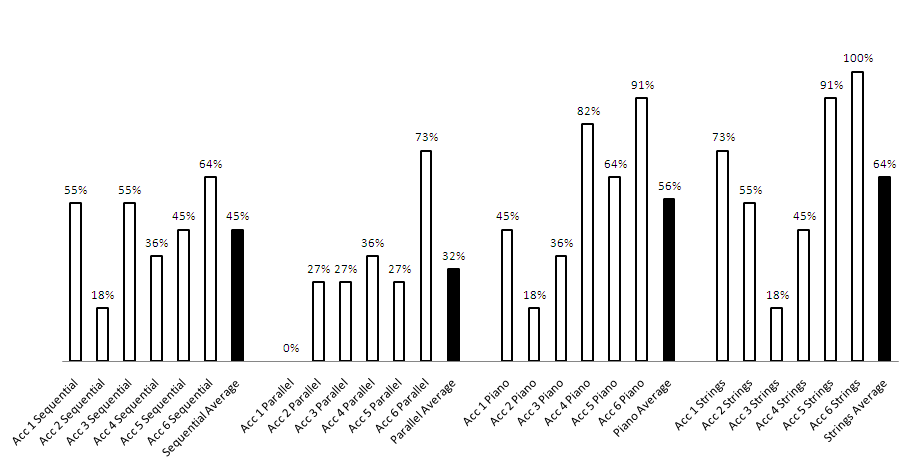
\includegraphics[scale=0.5]{agreegraph}
\caption{A graph showing the average amount that testers agreed with the expert's decision whether to invest in an account, not invest in an account or to remain undecided. (note that `strings' and `piano' are L-System generated sequences)}
\label{fig:agreegraph}
\end{figure}

\begin{figure}[ht]
\centering
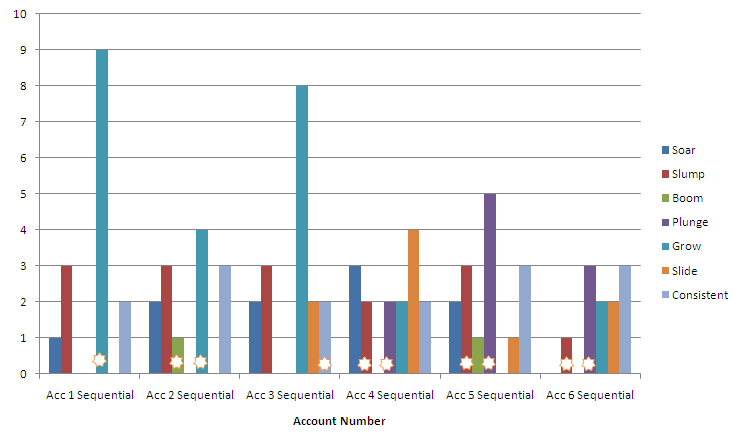
\includegraphics[scale=0.6]{agreegraphseq}
\caption{A graph showing how many times testers selected buzzwords for each account in the Signal Mapping Sequential output. A star designates that this option was selected by the expert.}
\label{fig:agreegraphseq}
\end{figure}

\begin{figure}[ht]
\centering
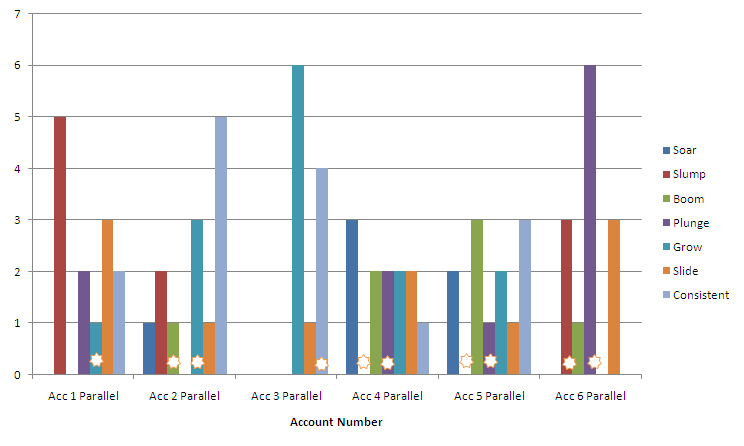
\includegraphics[scale=0.6]{agreegraphpar}
\caption{A graph showing how many times testers selected buzzwords for each account in the Signal Mapping Parallel output. A star designates that this option was selected by the expert.}
\label{fig:agreegraphpar}
\end{figure}

\begin{figure}[ht]
\centering
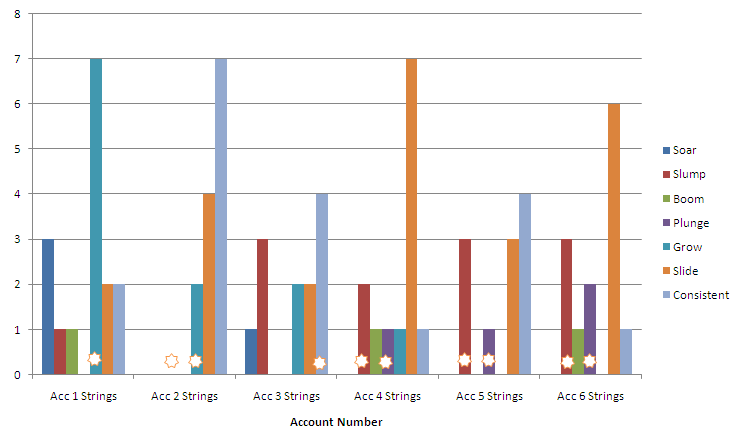
\includegraphics[scale=0.6]{agreegraphstrings}
\caption{A graph showing how many times testers selected buzzwords for each account in the L-System Strings output. A star designates that this option was selected by the expert.}
\label{fig:agreegraphstrings}
\end{figure}

\begin{figure}[ht]
\centering
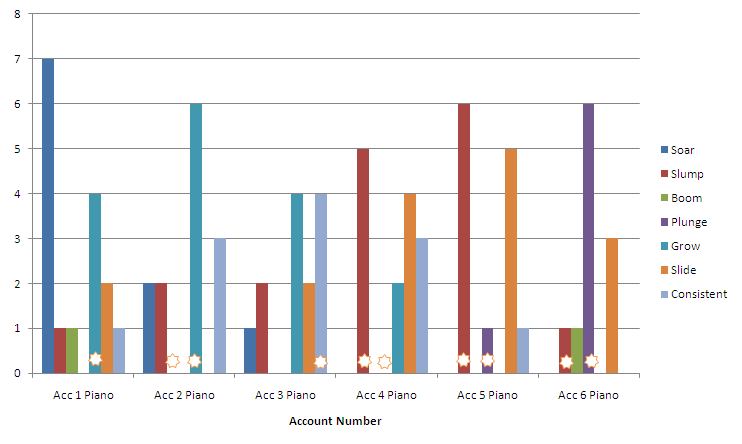
\includegraphics[scale=0.6]{agreegraphpiano}
\caption{A graph showing how many times testers selected buzzwords for each account in the L-System Strings output. A star designates that this option was selected by the expert.}
\label{fig:agreegraphpiano}
\end{figure}

\noindent The challenge of the evaluation was to deduce how often the testers agreed with the investment decisions of the expert. \textit{Figure \ref{fig:agreegraph}} shows on average how much agreement there was (recall that the choice was one of \textit{three categories}: Invest, don't invest or undecided).

Looking at the averages for each of the four output types, we see that the two L-System implementations (Strings \& Piano) were more successful than the two Signal Mapping implementations (Sequential \& Parallel).

We can gain more insight if we look at how spread out the opinions of the testers were for each of the output types. This can be done by calculating their standard deviations:

\begin{singlespace}
\begin{formality}
$\sigma_{Signal\_Mapping\_Sequential} = 0.162623126$ \\
$\sigma_{Signal\_Mapping\_Parallel} = 0.235312347$ \\
$\sigma_{L-System\_Piano} = 0.305595206$ \\
$\sigma_{L-System\_Strings} = 0.30424001$
\end{formality}
\end{singlespace}

We can see that the Signal Mapping outputs show less of a spread than the L-Sytem outputs. From this we might deduce that the L-System output types were more ambiguous than the Signal Mapping output types, and therefore the tester's investment choices were more varied. Why might this be? Consider that the Signal Mapping output types were composed of simple musical sequences (scales going up, etc). These movements are clear and were easier to interpret by the testers.

The L-System output types were generated from rules, and therefore produced sequences which were not as clear cut as an ascending scale might have been. This would mean that it was more difficult to arrive at a conclusion as to the state of the account.

That said, if the L-System output types were more ambiguous than the Signal Mapping output types, then why would it be that the L-System approach would fare better? Intuitively, we might assume that simpler musical sequences would be easier to interpret. In order to solve this mystery, we need to investigate further.

Recall that we used descriptive `buzzwords' as a way of evaluating the state of an account. Both the expert and the testers selected one or more words to describe each account (or account's output sequence) based on their perception. From \textit{figures \ref{fig:agreegraphseq}, \ref{fig:agreegraphpar}, \ref{fig:agreegraphstrings} and \ref{fig:agreegraphpiano}}  we can tell how often the testers chose the same descriptive words as the expert.

What we find with the two Signal Mapping implementations is that the testers were poor at correctly picking the same buzzwords as the expert. However, with the L-System implementation, the testers were better at selecting the same word.

As \textit{both} of the two implementations are based on the same derived signals, we can trace the difference down to the L-System processing. With the Signal Mapping implementation, musical sequences are produced mechanically by performing calculations. With the L-System implementation, we have a more organic process. This process appears on the surface to produce more complex music, but in fact we would suggest that biologically-inspired techniques are better able to tune the music towards the human ear.

\begin{figure}[ht]
\centering
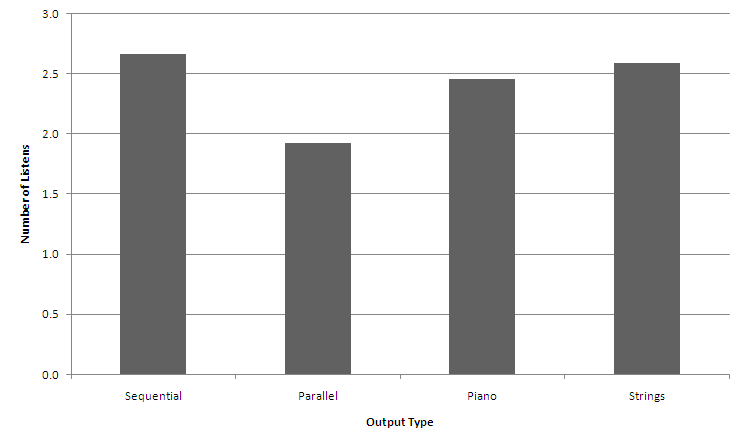
\includegraphics[scale=0.6]{numberoflistens}
\caption{A graph showing the average number of listens needed for each output type. (note that `strings' and `piano' are L-System generated sequences)}
\label{fig:numberoflistens}
\end{figure}

In terms of the average number of listens needed by each tester for each output type \textit{(figure \ref{fig:numberoflistens})}, there is an approximate correlation between the length of the sequence, and the number of listens needed \textit{(figure \ref{fig:numberoflistenscor})}. For example, a very short sequence (3 seconds) sometimes requires more listens than a longer piece (20 seconds). This is of interest to us, because the tempo reflects the amount of change in an account.

\begin{figure}[ht]
\centering
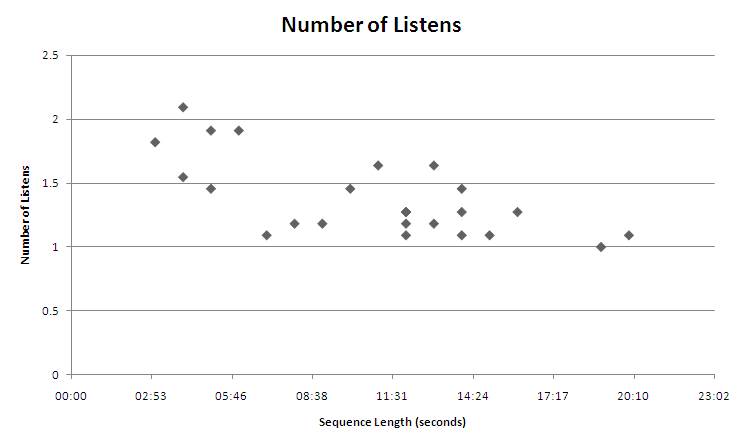
\includegraphics[scale=0.6]{numberoflistenscor}
\caption{A graph showing the correlation between the length of a musical sequence (in seconds) and the average number of listens that the tester needed.}
\label{fig:numberoflistenscor}
\end{figure}

This is also an unusual observation, because we might intuit that a short sequence would not need a further listen because it is simpler to analyse\footnote{The short-term memory model describes the way the human brain can record a small number of items in detail for up to 30 seconds. This would suggest that a shorter piece of music would be easy to hold in the mind than a longer one.}. As a concequence of this, we may wish to take into account that the tempo setting may have a side effect in the way the music was perceived by the tester.

But, what about the musicality of each approach? \textit{Figure \ref{fig:musicalityaverage}} shows how `musical' the tester considered each of the four types of output sequence to be, on a scale of 1 to 5. The two best achievers in this instance were the Sequential Signal Mapping and the Piano L-System.

\begin{figure}[ht]
\centering
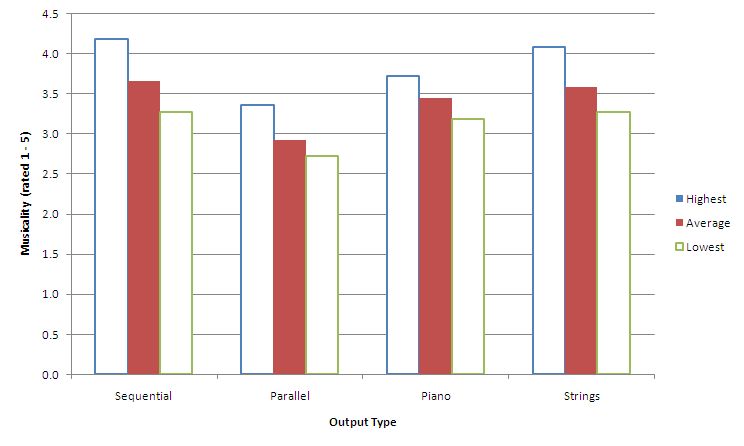
\includegraphics[scale=0.6]{musicalityaverage}
\caption{A graph showing the average spread of the musicality ratings given to each output type.}
\label{fig:musicalityaverage}
\end{figure}

Why was the prediction accuracy lower for the Signal Mapping Parallel output than it was for its Sequential counterpart? I would suggest that this is for three reasons. Primarily, we have several musical sequences playing concurrently in the Parallel output, which could make them difficult to tell apart. In the Sequential output, these sequences are played one after the other, in order of importance.

The second reason might be to do with the key shift which occurs in the Parallel output. Remember, that in order to avoid discordancy, all sequences are shifted into the same key for the Parallel output. In the Sequential output, sequences retain their own key, therefore giving them their own `flavour'.

The third reason I propose is that as the sequences are played one after another in the Sequential output, the tester was able to look at their relations to each other in a different way to having them played in parallel.  For example, key changes stand out between parts of the sequence. This perspective is lost in the Parallel output.

\section{Summary and Conclusions}

By looking at the results, we can see that \textbf{the music does to an extent represent the accounts they're generated from}. Additionally, we witness that the \textbf{L-System approach performs the best}, although both approaches do have their merits. We discovered that under ideal circumstances, testers will only correctly analyse the account from the music 64\% of the time.

\textbf{Testers considered the sequences they heard as music} (ie, have a high level of `musicality'). This is important, as one of the objectives of this project is to generate music from accounts. In this area, we can say that we have been successful.

We discovered that, paradoxically, adding an extra level of complexity to the music (via the L-System implementation) actually improves a person's ability to assess the account. This implies that the emergent properties displayed by the L-System make the nature of the accounts more clear. Perhaps it shouldn't be surprising that a biologically-inspired approach should work well when the subjects are biological!

What is really needed now is a way of formally defining the attributes in music in the same way that we can define attributes in the accounts. Achieving this would open up new avenues which would help us generate music which more closely represents the account, and it is this challenge we will attempt to meet in the next chapter.